%! Author = lazza
%! Date = 03/05/2022

\section{Static scheduling}\label{sec:static-scheduling}
Compilers can use sophisticated algorithms for code
scheduling to exploit ILP\@.
The amount of parallelism available within a \textbf{basic block}, a straight-line code sequence with no branches in
except to the entry and no branches out except at the
exit, is quite small (statistically it varies from 4 to 7 instructions).

Data dependence can further limit the amount of ILP we
can exploit within a basic block to much less than the
average basic block size.

To obtain substantial performance enhancements, we
must exploit ILP across multiple basic blocks (i.e.,
across branches).

Static detection and resolution of dependencies are accomplished by the compiler, dependencies are avoided by code
reordering.

The output of the compiler is a reordered dependency-free code, which can be processed, for example, by the VLIW (Very
Long Instruction Word) processors.

\paragraph{Limits of Static Scheduling}
\begin{itemize}
    \item unpredictable branches
    \item variable memory latency
    \item code size explosion
    \item compiler complexity
\end{itemize}

Till know we had a single-core multi-cycle parallelism, thanks to the single-issue pipelined architecture.
The single-issue architecture means we cannot aim to have an ideal CPI bigger than one.

Multi-issue architectures are the next step to improve the CPI:
\begin{itemize}
    \item Superscalar
    \item VLIW
\end{itemize}

\subsection{VLIW architectures}\label{subsec:vliw-architectures}
Each instruction word contains more than one operation, the processor can initiate multiple operations per cycle
specified completely by the compiler.
This leads to a low hardware complexity:
\begin{itemize}
    \item no scheduling
    \item reduced support of variable latency instructions
    \item single control flow (1 PC)
    \item explicit parallelism
\end{itemize}

An instruction can be a set of operations that are intended to be issued simultaneously, the VLIW has multiple
operations packed into one instruction, and each type of operation has its own slot.

\begin{figure}[h]
    \centering
    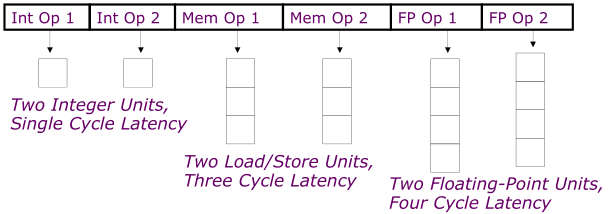
\includegraphics[scale = 0.4]{images/vliw}
    \caption{Very Long Instruction Word}
    \label{fig:vliw}
\end{figure}

This type of architecture requires guarantees of:
\begin{itemize}
    \item parallelism within an instruction does not generate RAW data hazard
    \item no data use before the data is ready, no data interlocks
\end{itemize}

Compiler responsibilities:
\begin{itemize}
    \item maximize parallel execution
    \begin{itemize}
        \item exploit ILP and LLP (Loop Level Parallelism)
        \item it is necessary to map the instructions over the machine functional units
        \item this mapping must account for time constraints and dependencies among the tasks
    \end{itemize}
    \item guarantee intra instruction parallelism
    \item avoid hazards (no interlocks), typically separates operations with explicit nops
    \item minimize the total execution time
\end{itemize}


\paragraph{Pros:}
\begin{itemize}
    \item[] simple HW
    \item[] good compilers can effectively detect parallelism
\end{itemize}
\paragraph{Cons:}
\begin{itemize}
    \item huge number of registers to keep active the FUs
    \begin{itemize}
        \item needed to store operands and results
    \end{itemize}
    \item large data transport capacity between
    \begin{itemize}
        \item FUs and register files
        \item Register files and Memory
    \end{itemize}
    \item high bandwidth between i-cache and fetch unit
    \item large code size
    \begin{itemize}
        \item use of (big) nops in the VLIW
        \item unpredictable branches have different optimal schedules that varies with branch path
    \end{itemize}
    \item knowing branch probabilities requires significant extra steps in build process due to profiling
\end{itemize}


An example of scheduling of a loop in VLIM architecture:
\begin{table}[h]
    \centering
    \begin{tabular}{c|c|c|c}
        \toprule
        operations & \textbf{ls, sd} & \textbf{add, bne} & \textbf{fadd} \\
        \midrule
        clock cycles & 3 & 1 & 4\\
        \bottomrule
    \end{tabular}
    \label{tab:}
\end{table}

\begin{figure}[h]
    \centering
    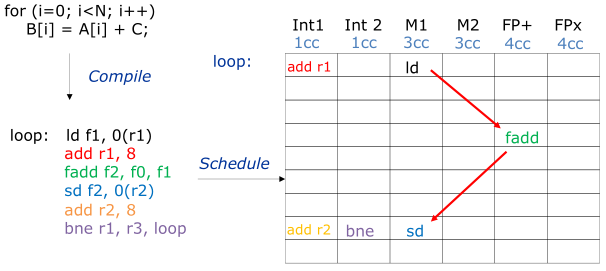
\includegraphics[scale = 0.4]{images/vliw-no-loop-unrolling}
    \caption{Loop execution on VLIM}
    \label{fig:vliw-no-loop-unrolling}
\end{figure}

Many blank lines in the scheduler corresponds to nops, leading to \(\frac{1\text{ FP ops}}{8\text{ cycles}} = 0,125\)
, which is far from our ideal CPI > 1.
To increase parallelism we use loop unrolling.

\clearpage
\subsection{Loop unrolling}
The idea is that we can extend the loop body as to include a finite number of subsequent iterations of the loop,
increasing the amount of available ILP\@.
Unrolling simply replicates the loop body multiple times, adjusting the loop termination code, by doing so the loop
\textit{overhead} decrease relatively to the loop \textit{body}.

\begin{center}
    Loop = (loop prolog + \(4\, \times\)\textit{loop body} + loop epilog) \texttimes $\, \frac{n}{4}$ iterations
\end{center}

\begin{figure}[h]
    \centering
    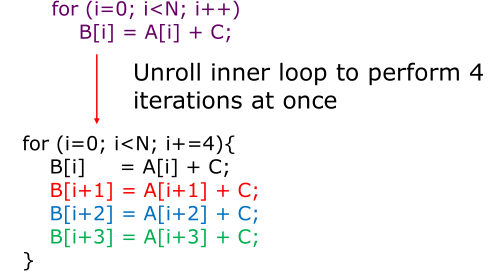
\includegraphics[scale = 0.4]{images/loop-unrolling-1}
    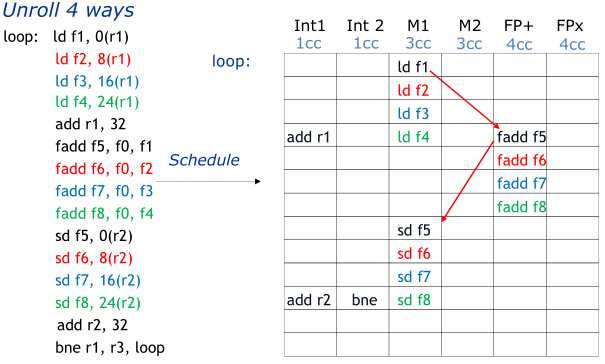
\includegraphics[scale = 0.4]{images/loop-unrolling-2}
    \caption{Loop unrolling}
    \label{fig:loop-unrolling}
\end{figure}

Note that non FP operations can have multiple schedule locations, e.g., the \verb|ld f2| could be scheduled also in
the first cycle to M2, but if does not decrease the CPI, it is recommended using a new instruction.
In this case we end up with \(\frac{4\text{ FP ops}}{11\text{ cycles}} \approx 0,36\), more than doubling the
previous result.

The \textbf{limits} of loop unrolling:
\begin{itemize}
    \item[] code size
    \item[] number of register
\end{itemize}
That is, we have an upper bound to the number of replications of the loop body, which has to be considered constant
in regard to the $\theta(n)$ loop iterations: we reduced the \textit{prolog} and \textit{epilog} of the loop by
a constant.

We can optimize the results of loop unrolling with \textbf{software pipelining}, further increasing the ILP\@.
\begin{figure}[h]
    \centering
    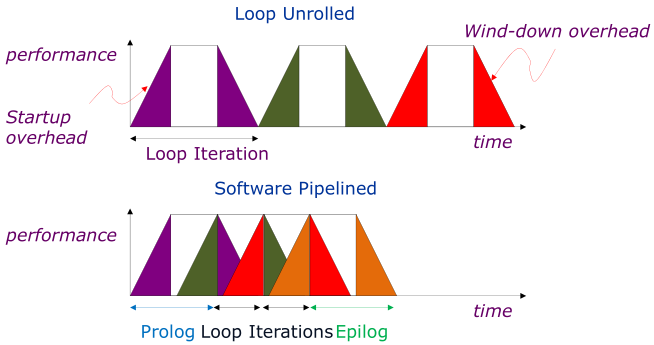
\includegraphics[scale = 0.4]{images/loop-unrolled-vs-software-pipelined-1}
    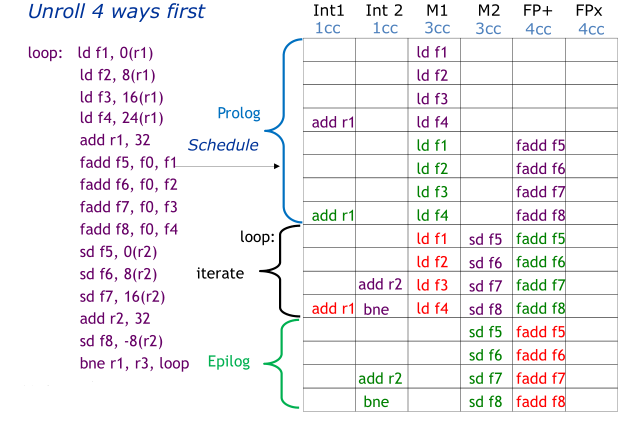
\includegraphics[scale = 0.4]{images/loop-unrolled-vs-software-pipelined-2}
    \caption{Loop unrolled vs Software pipelined}
    \label{fig:loop-unrolled-vs-sw-pipelined}
\end{figure}

\begin{center}
    Software Pipelined Loop = prolog + \textit{iterations} + epilog
\end{center}

In this case we have just one prolog and one epilog for all the loop iterations and can be considered $O(1)$ with
respect to the $n$ iterations.
For this reason we consider only the \textit{iterate} part for our performance evaluation which is \(\frac{4\text{ FP
ops}}{4\text{ cycles}} = 1\).

\textbf{Note:} in case of short loops, loop unrolling looses performance due to the costs of starting and closing the
iterations.

\clearpage
\subsection{Trace Scheduler}\label{subsec:trace-scheduler}
Loop unrolling is useful but does not cover other type of branches that limit the basic \textbf{block size} in
control-flow intensive irregular code.
In these cases is difficult to find ILP in individual basic blocks.

Trace scheduling focus on traces:
\begin{itemize}
    \item a loop-free sequence of basic blocks embedded in the control flow graph
    \item it is an execution path which can be taken for some set of inputs
    \item the chances that a trace is actually executed depends on the input set that allows its execution
\end{itemize}

\textbf{Note:} a trace may include branches but not loops.

\paragraph{Algorithm} Idea, some traces are executed much more frequently than others:
\begin{itemize}
    \item pick string of basic blocks, a trace, that represents most frequent branch path
    \item use profiling feedback or compiler heuristics to find common branch paths
    \item schedule whole "trace" at one
    \item add fixup code to cope with branches jumping out of trace
\end{itemize}
\begin{figure}[h]
    \centering
    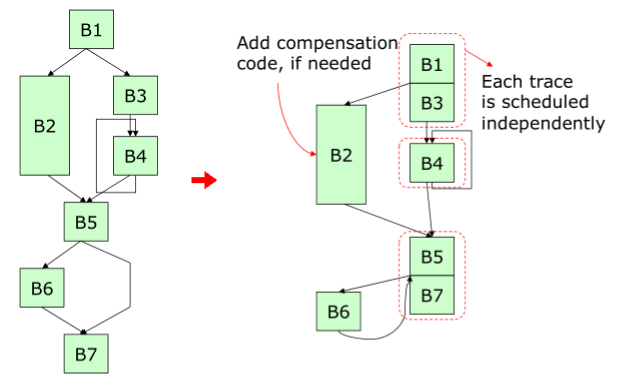
\includegraphics[scale = 0.45]{images/trace-scheduling}
    \caption{Trace scheduling}
    \label{fig:trace-scheduling}
\end{figure}

For example we suppose that \{B1, B3, B4, B5, B7\} is the most frequently executed path, therefore the traces are
\{B1, B3\}, \{B4\} and \{B5, B7\}.\\
\textbf{Note:} Traces are scheduled as if they were basic blocks, by removing control hazards we increase ILP\@.

\paragraph{Problems} Compensation codes are difficult to generate, especially entry points (of a different path).
In addition to need of compensation codes there are
restrictions on movement of a code in a trace:
\begin{itemize}
    \item \textbf{dataflow} of the program must not change, it is guaranteed to be correct by maintaining:
    \begin{itemize}
        \item data dependencies
        \item control dependencies
    \end{itemize}
    \item the exception behaviour must be preserved
\end{itemize}


\paragraph{Solutions}There are two approaches to eliminate control dependency:
\begin{itemize}
    \item use of \textbf{predicate} instructions (Hyperblock scheduling).
    Useful for mispredicted branches that limits ILP\@.
    \item use of \textbf{speculative} instructions (Speculative Scheduling), and speculatively move an instruction
    before the branch.
    Useful for scheduling long latency loads early.
\end{itemize}

\begin{figure}[h]
    \centering
    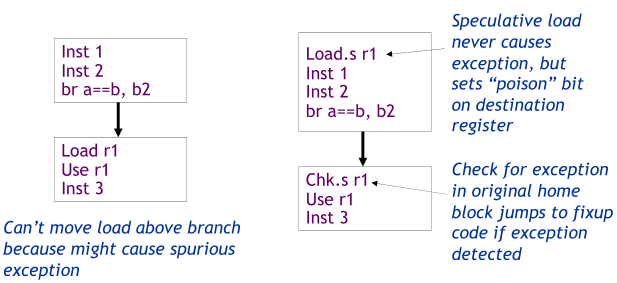
\includegraphics[scale = 0.4]{images/speculative-instruction}
    \caption{Speculative instruction}
    \label{fig:speculative-instruction}
\end{figure}


\begin{figure}[h]
    \centering
    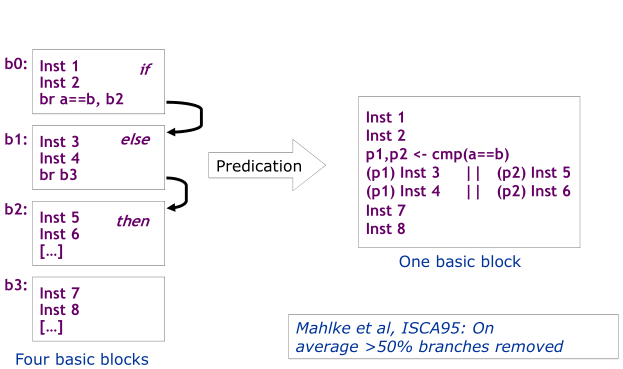
\includegraphics[scale = 0.4]{images/predicated-execution}
    \caption[Predicated execution]{Predicated execution}
    \label{fig:predicated-execution}
\end{figure}



\subsection{Rotating Register Files}\label{subsec:rotating-register-files}
Scheduled loops require lots of registers, lots of duplicated code in prolog and epilog.
\textbf{Solution}: allocate new set of registers for each loop iteration.

\textbf{Rotating Register Base} (RRB) register points to base of current register set.
A value is added to the \textit{logical} register specifier to give \textit{physical} register number.

\begin{figure}[h]
    \centering
    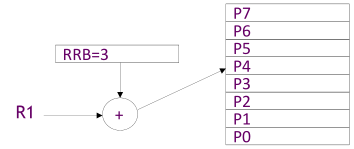
\includegraphics[scale = 0.4]{images/rotating-register-file-1}
    \caption{Rotating Register Base}
    \label{fig:rotating-register-base}
\end{figure}

If we know the clock cycles that each operation takes we can use rotate new register by
\begin{center}
    \textit{\#logical R} = \textit{\#physical R} $+$ (\#iteration \(\mod\) \#clock cycles required)
\end{center}

\begin{figure}[h]
    \centering
    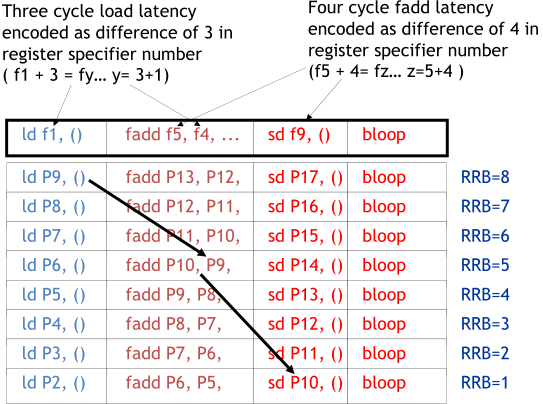
\includegraphics[scale = 0.4]{images/rotating-register-file-2}
    \caption{Rotating registers}
    \label{fig:rotating-registers}
\end{figure}